\documentclass[10pt,conference]{IEEEtran}

\usepackage{url}
\usepackage{cite}
\usepackage{graphics}
\usepackage{graphicx}
\usepackage{epsfig}
\usepackage{amssymb}
\usepackage{amsthm}
\usepackage{lineno}

\hyphenation{op-tical net-works semi-conduc-tor}

\begin{document}
\title{ADHOP: an Energy Aware Routing Algorithm for Mobile Wireless Sensor Networks}

\author{
    \IEEEauthorblockN{Alexandre Massayuki Okazaki and Ant\^onio Augusto Fr\"ohlich}
    \IEEEauthorblockA{
        Laboratory for Software and Hardware Integration (LISHA)\\
            Federal University of Santa Catarina (UFSC)\\
            P.O.Box 476, 88040900 -- Florian\'opolis -- Brazil\\
            \{alexandre,guto\}@lisha.ufsc.br
    }
}

\maketitle

\begin{abstract}
Sensor nodes usually propagate data packets in a multihop fashion.
However, in the most of routing protocols, the optimal routes are likely to be used for the following transmissions.
As a result, the optimal routes tend to accelerate the energy depletion of nodes, especially in low-power networks, which are noisy and error-prone.
ADHOP is a low overhead routing algorithm which can adapt to dynamic topologies.
Such protocol is designed to use metrics as heuristic information to support routing decisions according to the network needs, such as distance, latency, residual energy, and/or signal strength.
Our approach aims at using residual energy as a metric in ADHOP to distribute the network traffic load, thus balancing the energy consumption among nodes without compromising communication.
Such method also allows us to achieve a routing algorithm powerful enough to reduce the energy consumption per delivered data in high data loss scenarios.
\end{abstract}

\IEEEpeerreviewmaketitle

\section{Introduction}
\label{introduction}

Sensor node typically features an embedded processor, a limited memory, and a low-power wireless radio \cite{Matrouk:2009}.
Furthermore, such devices are typically battery powered, thus imposing several restrictions on the design of protocols for WSNs \cite{Zeng:2009,Anastasi:2009}, from the physical to the application layer.
Maximizing the network lifetime and balancing the energy consumption have raised some attention and effort on several approaches of routing in Wireless Sensor Networks (WSNs).
Hence, many proposals for routing protocols have specifically been made to handle energy depletion, although few consider mobile sensor nodes \cite{Shuang:2009, Hu:2009}.
However, dealing with the limited energy resources of sensor nodes, in mobile WSNs, becomes a considerable challenge in the design of routing protocols.

Ant-based routing algorithms use pheromone to learn and adapt routes in relatively short periods.
Nevertheless, most of them are not suitable for low-power wireless networks \cite{Shuang:2009}.
Such algorithms typically use control packet transmissions in order to keep the pheromone information updated and to establish reliable data delivery ratio.
However, in WSNs, a routing protocol must avoid additional routing overhead as much as they must distribute the load transmission over the network in order to save residual energy in the nodes.
Therefore, energy aware routing protocols must dynamically handle network topology changes while they must also be energy efficiency.

In this work, we introduce an energy aware \emph{Ant-based Dynamic Hop Optimization Protocol} (ADHOP), a self-configuring and multihop reactive routing protocol which aims at providing a low-overhead routing for mobile WSNs.
Our approach uses the ant collective behavior to make routing decisions by pheromone and heuristic information.
By using pheromone, ADHOP can adapt to network changes, such as mobility and node failures.
In fact, ADHOP is designed to use one or more heuristic information to support routing decisions according to the network needs, such as distance, latency, residual energy, and/or \emph{Received Signal Strength Indicator} (RSSI).
Our approach aims at using residual energy information to distribute the network traffic load, thus reducing the energy consumption per delivered data.

The rest of the paper is organized as follows.
The related works are introduced in section \ref{related_work}.
We describe and explain our proposal in section \ref{proposed}.
In section \ref{evaluation}, we analyze and evaluate the energy aware ADHOP.
Finally, section \ref{conclusion} presents our conclusions.

\section{Related Work}
\label{related_work}

Vlajic and Stevanovic \cite{Vlajic:2009} analyzed the pros and cons of deploying path-constrained mobile sinks in real IEEE 802.15.4 networks.
They introduced two basic mechanisms for the reduction of mobility-related overhead in WSNs.
They also demonstrated analytically and through simulation that, in idealist networks, mobile sinks can result in a better distribution of routing load and longer network lifetime.
Unfortunately, in networks, including IEEE 802.15.4, the overhead is not zero.
These networks use mechanisms that generate additional overhead to manage congestion, lessen mobility, and consequently bring down the amount of changes in network topology.
Hence, for contemplating the use of real WSNs with continuous changes in network topology, the minimization of protocol overhead may have to be the first course of action.

\emph{Geographic Routing with Environmental Energy Supply} (GREES) is an algorithm that makes routing decisions combining geographic and energy efficient routing techniques \cite{Zeng:2009}.
It takes into account the realistic wireless channel condition, residual energy level, and environmental energy supply.
GREES aims at directing data packets along low cost links while balancing the energy consumption in nodes with environmental energy supply.
Different from our proposal, GREES maintains some information about the neighborhood such as location, residual energy, energy harvesting ratio, energy consumption ratio, and link quality.
However, keeping all these information about neighbor nodes sufficiently updated, to ensure maximum data delivery ratio, brings additional overhead to the network.

Patel and others \cite{Kumar:2010} proposed a coverage and connectivity aware neural network based on energy efficient clustering routing algorithm for WSNs.
It aims to maximize the network lifetime through a problem formulated as \emph{linear programming} with connectivity and coverage aware constraints.
Hence, the routes are distributed to prevent depletion of the most frequently used nodes.
The authors also proposed the use of neural networks in the election of cluster heads according to the residual energy of network nodes.
The proposed scheme is highly effective for data delivery ratio.
Different from our proposal, this algorithm requires prior knowledge of the network and the residual energy in each of the possible routes to a certain destination.
On high-scalability networks, the number of route options tends to increase, thus increasing the routing overhead.

Chen and others \cite{Shuang:2009} proposed \emph{Ant-Based On-Demand Energy Route} (AOER) protocol.
The authors focused on the design of a routing algorithm for IEEE 802.15.4 mesh networks.
Different from other protocols based on ACO, AOER requires less memory storage and less processing power.
It also uses simpler data structures for ants and routing table.
The algorithm maintains the routes by inserting pheromone according to the residual energy in the nodes in order to distribute the traffic in the network equally.
AOER has shown satisfactory results in prolonging the network lifetime and balancing energy consumption among nodes.
The authors present a solution similar to our approach taking into account the reduction of memory and processing.
However, AOER uses a means to reduce the energy consumption, which brings down the data delivery ratio.

\section{ADHOP: The Proposed Routing Strategy}
\label{proposed}

ADHOP is a self-configuring and multihop reactive routing protocol that aims at providing routing aware of the network flow for mobile WSNs \cite{OkazakiB:2011}.
It is a routing protocol which uses pheromone as a metric to make routing decisions in dynamic topologies.
ADHOP has obtained satisfactory results in terms of data delivery ratio, routing overhead, and congestion avoidance for environments of dynamic topology \cite{OkazakiB:2011}.

ADHOP aims at minimizing the routing overhead without compromising the data delivery ratio.
Furthermore, because of \emph{Ant Colony Optimization} (ACO), ADHOP can handle problems in \emph{ad hoc networks} and dynamic network topologies to avoid congestion, broken routes, and improve the discovery and maintenance of routes.
In our approach, all routing decisions are made locally, without needing the knowledge of the network to route data.
Each node stores an amount of pheromone between itself and any other node in the network.
As a result, ADHOP pheromone concentration and evaporation rates are adjusted dynamically considering global information collected and disseminated by ants.

ADHOP ants are able to use local information that encompasses resource availability and other heuristic information, such as distance, latency, and residual energy, as shown in Figure \ref{heuristics}.
A node forwarding too many packets adjust the pheromone to favor other routes, which resources are not being drained too quickly.

\begin{figure}[htbp]
\centering
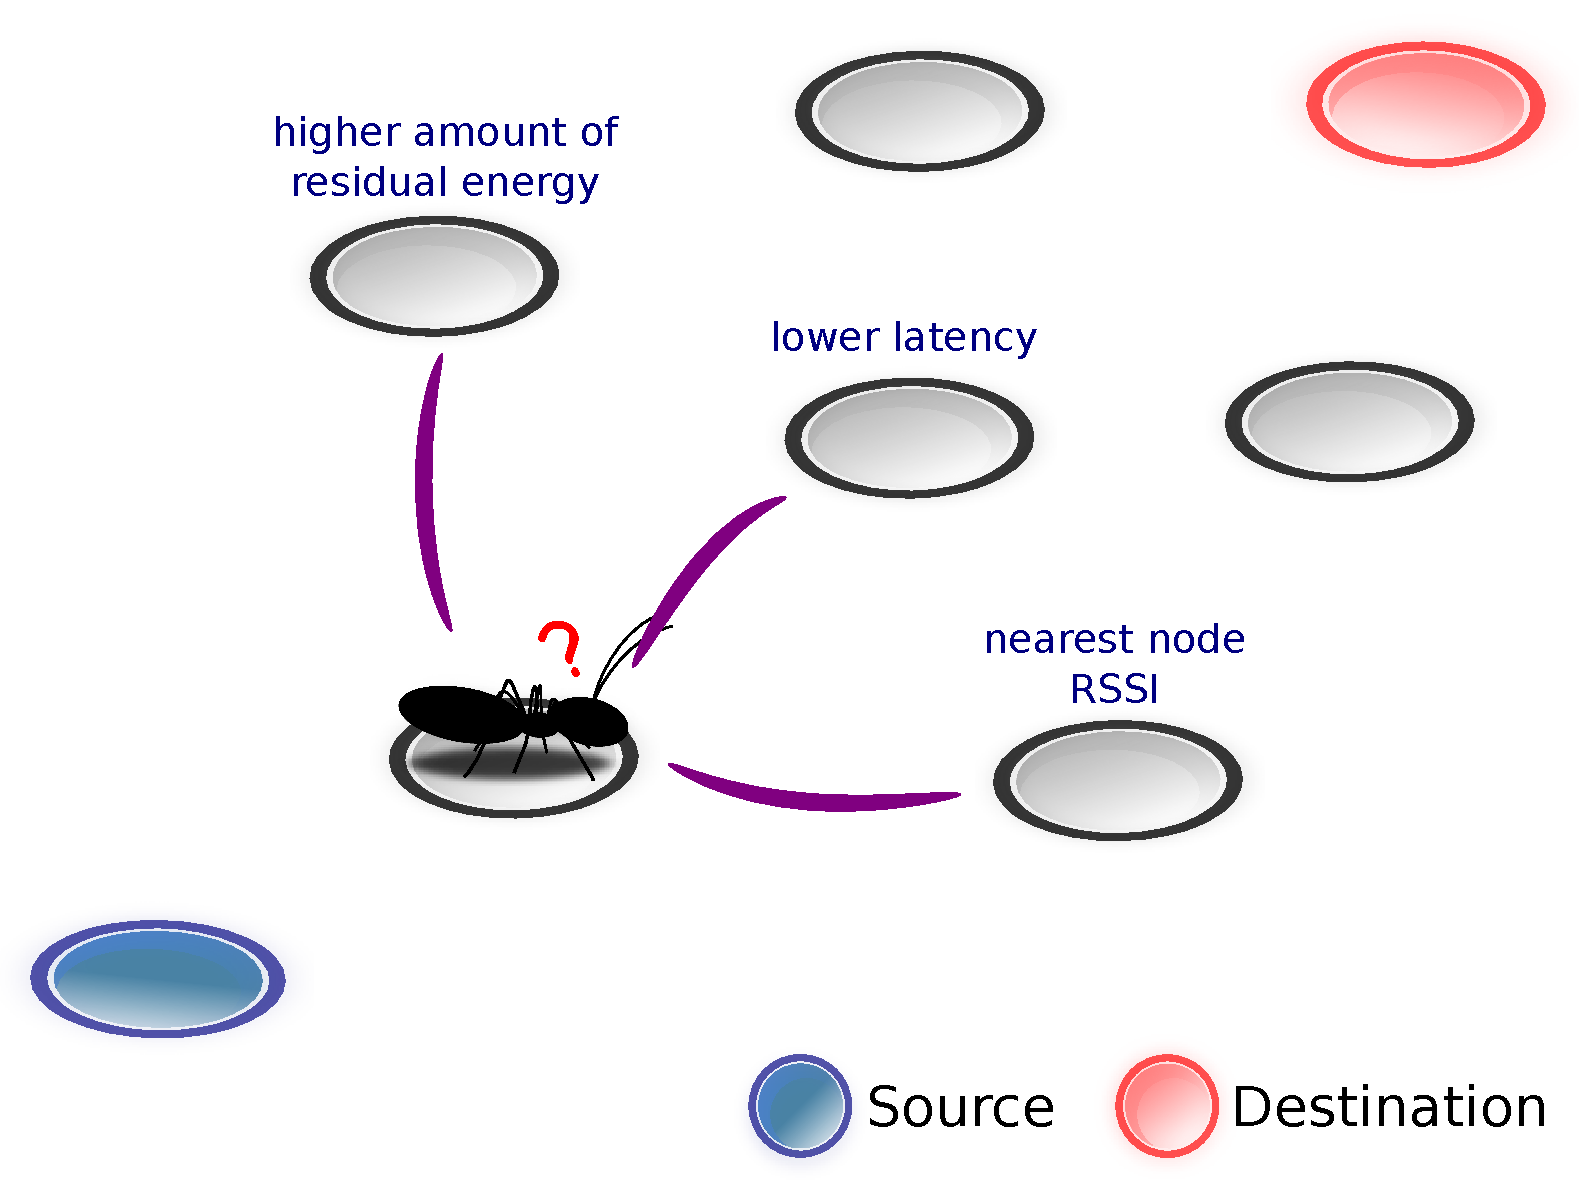
\includegraphics[width=220pt]{fig/ant_heuristic.pdf}
\caption{ADHOP Heuristics.}
\label{heuristics}
\end{figure}

Ant-based routing protocols can thereby maintain the routing table updated efficiently due to the proportionate dynamism of ants to detect changes in the network topology.
In order to make routing decisions properly, the ants are responsible for dissipating their knowledge of the network to obtain the best routes.
Therefore, the nodes do not need to be concerned to discover and maintain entire routes to the destination nodes.
They only need to direct the ant to the next hop toward the destination node through a local decision based on the source and destination node.

In mobile sensor networks, nodes may fail or move away from their routes.
As a result, if a part of the route is no longer used then the other nodes eventually leaves the route due to pheromone evaporation.
In ADHOP, the routes are not predetermined, and the hops are chosen dynamically at each node toward the destination.
Hence, our approach adapts to topology changes and network needs transparently, as shown in Figure \ref{back_2}.

\begin{figure}[htbp]
\centering
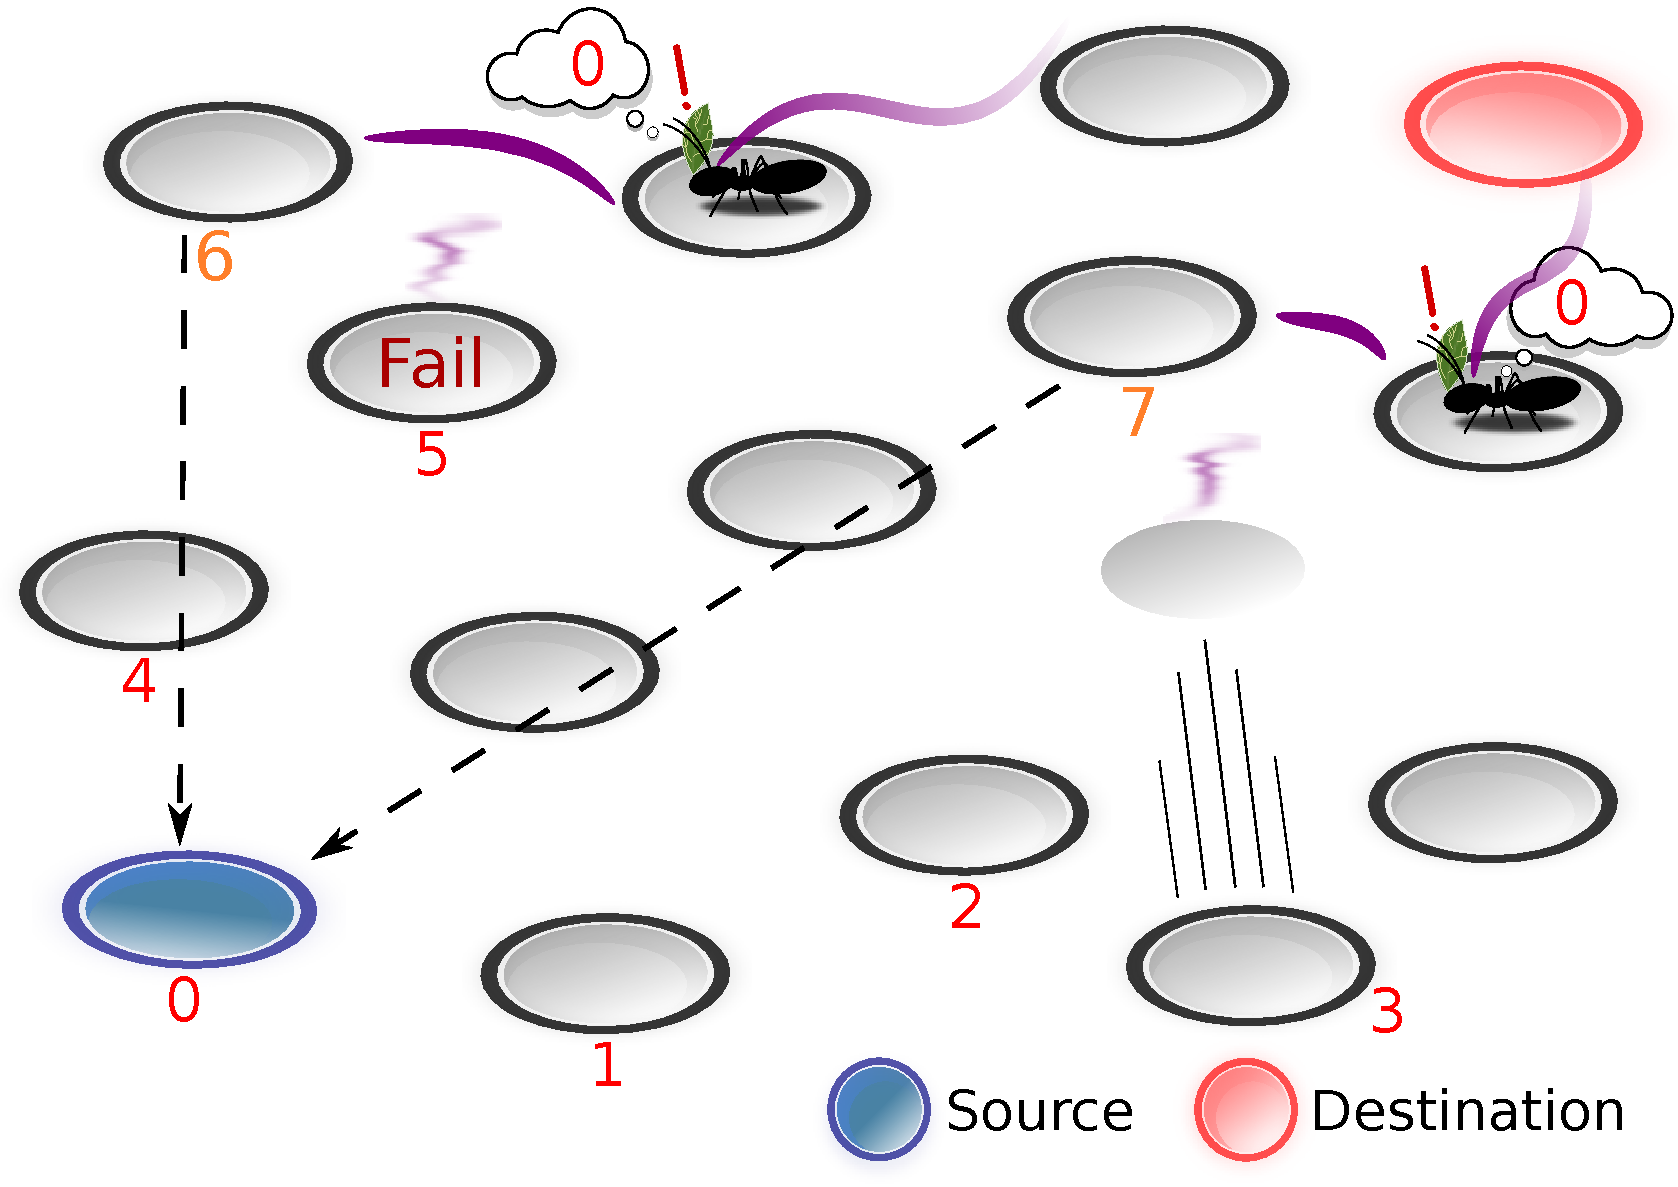
\includegraphics[width=220pt]{fig/ant_back-2.pdf}
\caption{Failed nodes and mobility, choosing an alternative path}
\label{back_2}
\end{figure}

ADHOP uses a routing table structure similar to the AOER inverted table which proves to be efficient to deal with pheromone \cite{Shuang:2009}.
Its operations are simpler and faster, and routes do not need to be stored entirely.
In order to accomplish these operations, ADHOP presents its own collection of ants: \emph{forward transport ant} (FTA) and \emph{exploratory transport ant} (ETA) \cite{OkazakiB:2011}.

In order to ensure that sudden changes in the network do not interfere the data transportation, both FTA and ETA perform data delivery while they deposit pheromone on the route which they travel.
These changes in topology are observed unwittingly by ants.
The data packet may thereby be dynamically redirected to a safer route.
Thereupon, warning messages or control packets are unnecessary.
This also means less control packets in the network, since the routing table does not need to be updated at each change in network topology.

ETAs are solely responsible for discovering routes to unknown nodes.
This ant randomly travels the network to reach the destination node.
At the destination, ETA delivers the data packet and returns to the source node.
On the way back, the ant just reinforces the pheromone trail.
The following data packet transmissions are performed by FTAs until the total evaporation of the pheromone on the route.
Nevertheless, at any time, if any route to any destination breaks, then any node on the route can use an ETA to recover or discover a new path.
It allows us to deal with dynamic network topologies and avoid as much as possible broken routes.

Each ant selects a node $v_{j}$ as the next hop from the current node $v_{i}$.
Actually, $v_{j}$ is the neighbor node which has a greater amount of pheromone.
At the node $v_{j}$, the ant updates the pheromone $\tau _{i,s}$ on the entry $\left ( v_{i},v_{s} \right )$ in the routing table, where $v_{s}$ is the source node, as follows \cite{Dorigo:2006}:
\begin{equation} \tau _{i,s} = \left ( 1 - \varphi \right ) \cdot \tau _{i,s} + \varphi \cdot \tau _{0} \label{adhop_pheromone_increasing} \end{equation}
where $\varphi \in \left [ 0,1  \right ]$ is pheromone decay coefficient, and $\tau _{0}$ is the initial value of pheromone.
This equation allows us to diversify the search process by decreasing the pheromone amount in the routes while allowing other ants to achieve different routes.
It also helps to increase the effect of different heuristics.

In ADHOP, the evaporation can occurs periodically to all nodes in the network, using the following equation \cite{Dorigo:2006}:
\begin{equation} \tau _{i,j} = \left ( 1 - \rho \right ) \cdot \tau _{i,j} , \quad \forall i \in N, \quad \forall j \in Z \label{adhop_evaporation} \end{equation}
where $\rho \in \left [ 0,1  \right ]$ is the evaporation rate, $N$ is the set of neighbor nodes, and $Z$ is the set of nodes which, together with neighbor nodes, define entries $\left ( v_{i},v_{j} \right )$ in the routing table.

Equations (\ref{adhop_pheromone_increasing}) and (\ref{adhop_evaporation}) allows us to use several heuristics to perform the routing (e.g., as shown in Figure \ref{heuristics}).
The pheromone decay coefficient ($\varphi$) and the evaporation rate ($\rho$) can be calculate using heuristic information, such as residual energy and data latency.
Such method improves the routing in terms of which heuristic is needed.

\section{Performance Evaluation}
\label{evaluation}

The implementations were performed using the OMNeT++ simulator.
It is an extensible, modular, component-based C++ simulation library and framework for building network simulators, and useful while modeling wireless communication.

Table I shows the OMNeT++ simulation parameters for a IEEE 802.15.4 network.
Each simulation scenario was run for a total of 900 seconds in an environment of high mobility that is conducive to high data loss.
The nodes are placed randomly in a rectangular area of 1200 meters x 1200 meters, and each one moves at a maximum speed of 5 meters per second, according to the Mass Mobility algorithm.
The data traffic is generated from 20 mobile source nodes to other 20 mobile sink nodes.
This base scenario was used for the experiments on OMNeT++.
The test scenarios are obtained by varying the heuristic information of ADHOP, and the number of nodes, ranged from 20 to 200.

\begin{table}[htbp]
\centering
\caption{OMNeT++ Configuration}
\begin{tabular}{l|r}
\hline \hline
\multicolumn{2}{l}{\bf{Parameter}}  \\
\hline
App. Msg. Length            & $32 B$            \\
App. Msg. Frequence         & $2 s$             \\
UDP Header Length           & $8 B$             \\
IP Header Length            & $20 B$            \\
Netmask                     & $255.255.0.0$     \\
ADHOP Header Length         & $20 B$            \\
IEEE 802.15.4 ACK           & True              \\
IEEE 802.15.4 Header Length & $22 B$            \\
IEEE 802.15.4 Max Frame Size& $102 B$           \\
Phy. Transmitter Power      & $1 mW$            \\
Phy. Sensitivity            & $-85 dBm$         \\
Phy. Thermal Noise          & $-110 dBm$        \\
Channel Carrier Frequency   & $2.4 GHz$         \\
Battery Capacity            & $850 mAh$         \\
Battery Voltage             & $3 V$             \\
Usage Radio Sleep           & $0.001 mA$        \\
Usage Radio Rx              & $22 mA$           \\
Usage Radio Tx              & $29 mA$           \\
\hline
\end{tabular}
\end{table}

In such scenario, our approach that uses residual energy as metric can reduce the average energy consumption by approximately $6\%$ compared to the ADHOP which uses latency as metric, as shown in Figure \ref{consumption}.
The energy aware approach can also reduce approximately $7\%$ compared to AODV. 
AOER is an efficient energy aware routing protocol for ad hoc networks, which reduces the average power consumed by approximately $13\%$ compared to our approach.

\begin{figure}[htb]
\centering
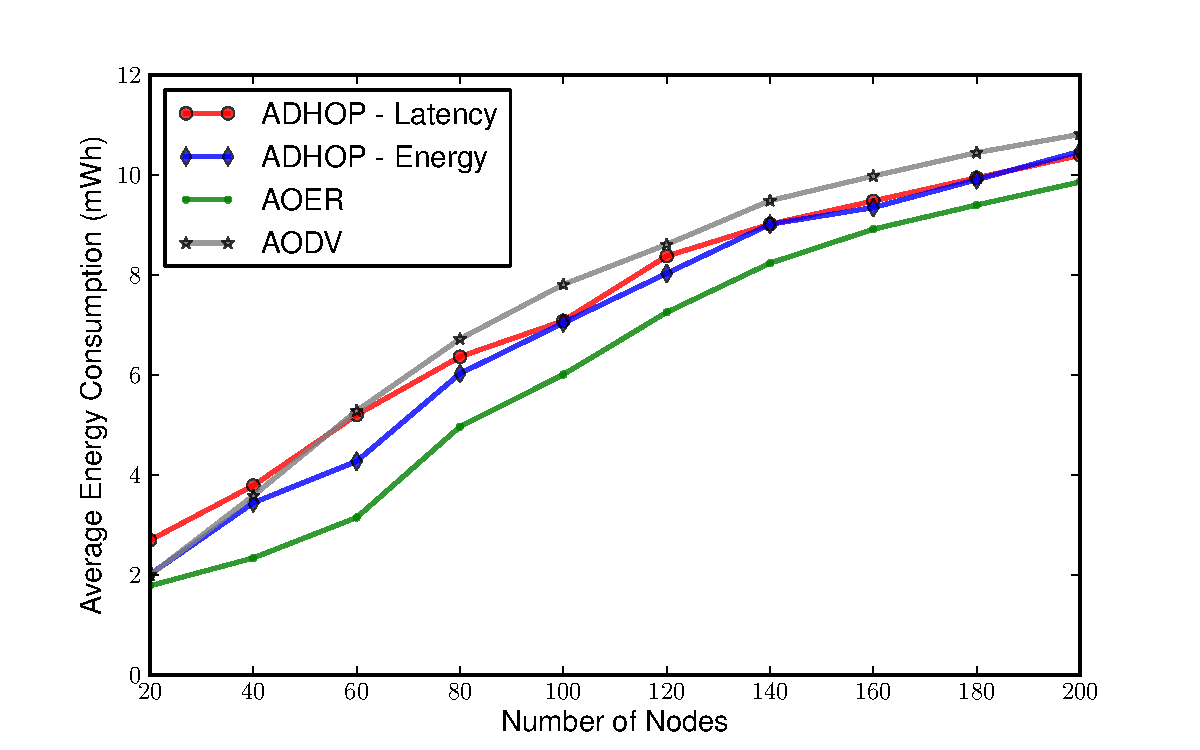
\includegraphics[width=260pt]{fig/average_consumption.pdf}
\caption{Average Energy Consumption}
\label{consumption}
\end{figure}

Figure \ref{standard_deviation} shows the standard deviation of nodes' energy consumption after 900 seconds of intense data transmission.
On average, energy aware ADHOP improves the balance of energy consumption by approximately $23\%$ compared to the ADHOP which uses latency as metric.

\begin{figure}[htb]
\centering
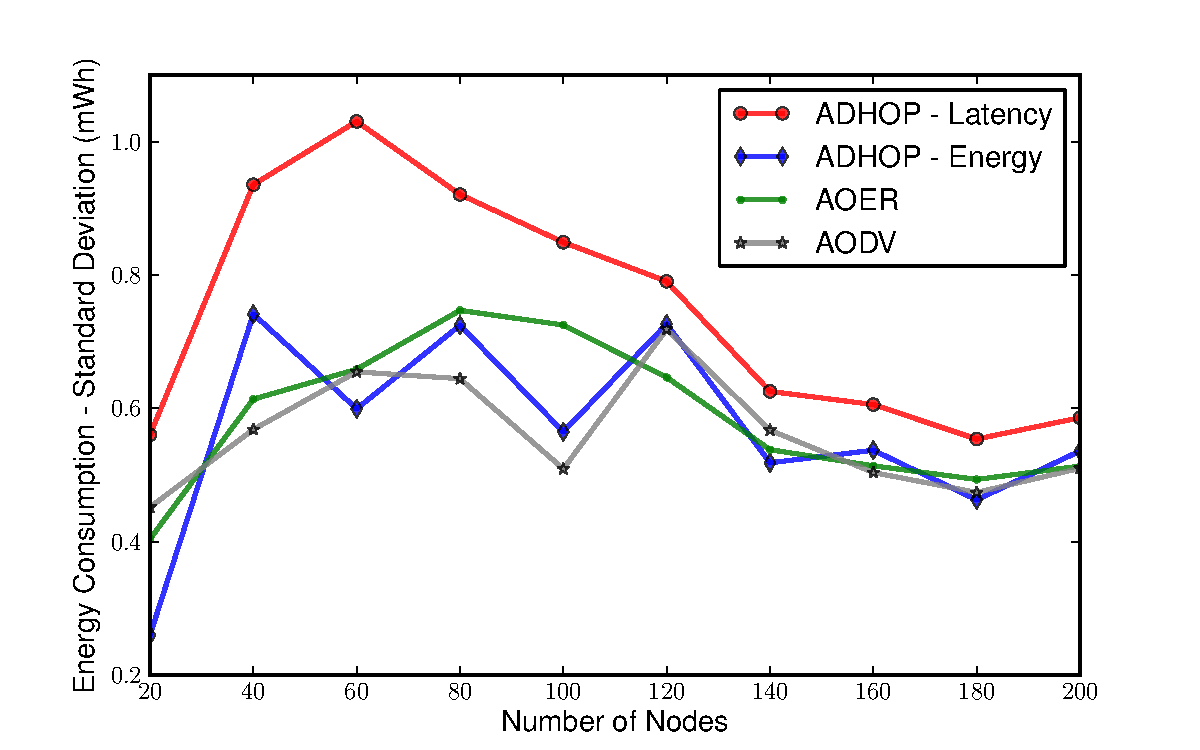
\includegraphics[width=260pt]{fig/standard_deviation.pdf}
\caption{Standard Deviation - Energy Consumption}
\label{standard_deviation}
\end{figure}

Although AOER has better average energy consumption, our approach produces better results in the energy consumption per delivered data by approximately $89\%$, as shown in Figure \ref{relation}.
We can notice that energy aware ADHOP can improve energy use while reducing the energy consumption without compromising data delivery ratio.
Differently from AOER, which has an aggressive method to reduce the energy consumption, thus affecting the data delivery ratio.
Such method is worsened due to the bit rate of IEEE 802.15.4 nodes which makes the connectivity worse in higher speeds \cite{Zen:2008}.
This means greater competition for the medium implying in collisions, congestions, data loss, and greater energy consumption for mobile, dense, and scalable networks, causing the depletion of energy on the routes.

\begin{figure}[htb]
\centering
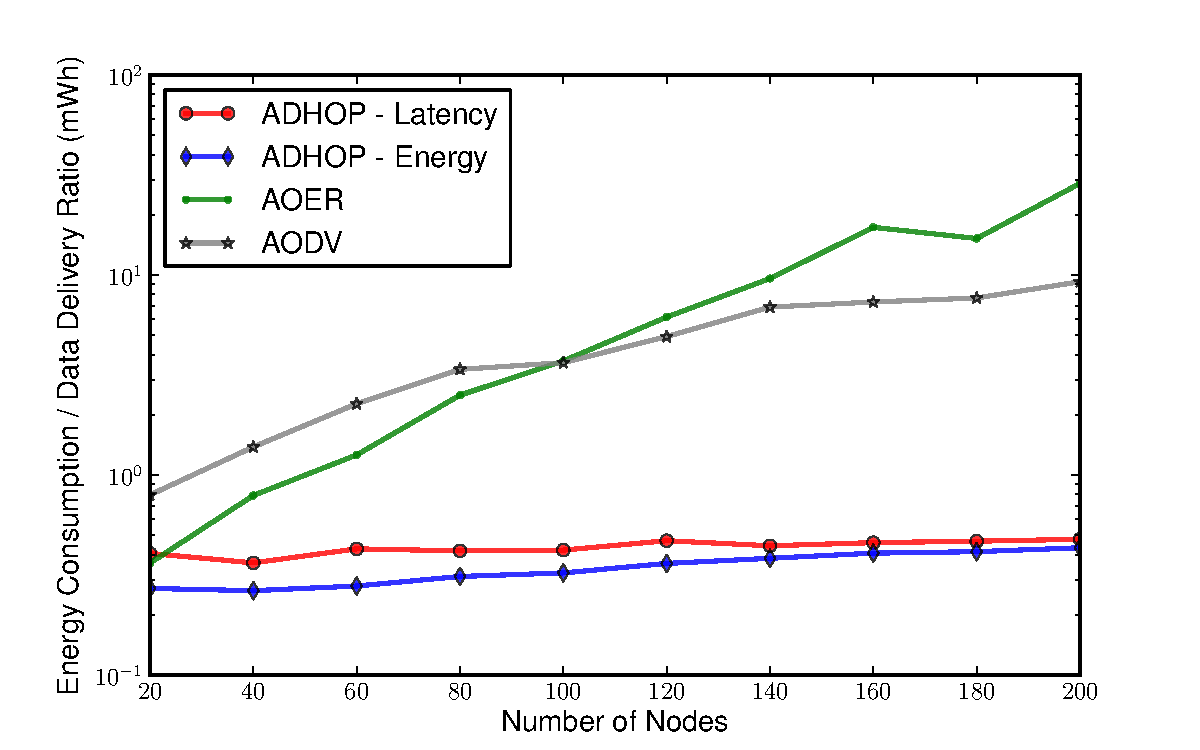
\includegraphics[width=260pt]{fig/relation.pdf}
\caption{Energy Consumption per Delivered Data.}
\label{relation}
\end{figure}

\section{Conclusion}
\label{conclusion}

In this paper, we proposed ADHOP, an energy aware routing algorithm that makes routing decision through the ACO metaheuristic.
ADHOP uses pheromone as a metric and residual energy as heuristic information to make routing decisions.
Our proposal aims at reducing the amount of control packets from the network and requiring less effort in communication, consequently in energy consumption.
ADHOP usually tends to accelerate the energy depletion of nodes in the optimal route.
Nevertheless, by using energy information as heuristic, the ants privilege sensor nodes with larger residual energy by increasing a larger amount of pheromone.
It also maximizes the probability of choice of routes with higher residual energy, thus balancing the energy consumption of the network.
Such heuristic allows us to handle energy depletion the way that complex operations in the network can be avoided.
Hence, while the energy consumption is balanced over the network, the network traffic is distributed, thus reducing the possibility of congestion.
We have shown through experiments in IEEE 802.15.4 networks that our proposal achieves satisfactory results in the energy consumption per delivered data in a mobile environment.

\bibliographystyle{IEEEtranS}
\bibliography{paper}

\end{document}

